\chapter{Methods}

\section{ANNISA FATHORONI/1164067}
\subsection{Teori}
Penyelesaian Tugas Harian 5 ( No. 1-6 )
\begin{enumerate}
\item Random Forest Dan Ilustrasi Gambarnya
\begin{itemize}
\item Pengertian Random Forest:

Random forests atau random decision forests adalah metode pembelajaran ensembel untuk klasifikasi, regresi dan tugas-tugas lain yang beroperasi dengan membangun banyak pohon keputusan pada waktu pelatihan dan menghasilkan kelas yang merupakan mode kelas (klasifikasi) atau prediksi rata-rata (regresi) dari masing-masing pohon. Random decision forests tepat untuk kebiasaan pohon keputusan 'overfitting' pada set pelatihan mereka.

\item Ilustrasi Gambar Random Forest :

\begin{figure}[ht]
\centering
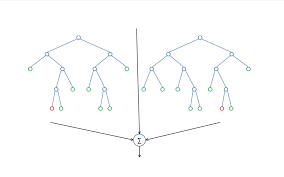
\includegraphics[scale=0.5]{figures/Chapter3AnnisaFathoroni1.png}
\caption{Random Forest}
\label{contoh}
\end{figure}

\end{itemize}

\item Cara Membaca Dataset

Berikut adalah cara membaca dataset :
\begin{itemize}
\item Buka Anaconda Navigator lalu jalankan Syder, kemudian import libraries yang dibutuhkan.
\item Masukkan kode python untuk membaca file csv, lalu jalankan

\begin{figure}[ht]
\centering
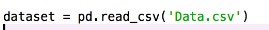
\includegraphics[scale=0.8]{figures/Chapter3AnnisaFathoroni5.jpeg}
\caption{Code Python}
\label{contoh}
\end{figure}

\item Maka pada window console akan menampilkan pesan berikut:

\begin{figure}[ht]
\centering
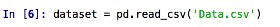
\includegraphics[scale=0.8]{figures/Chapter3AnnisaFathoroni6.jpeg}
\caption{Output}
\label{contoh}
\end{figure}

\item Dari explorer dapat terlihat dataset yang terimport.

\begin{figure}[ht]
\centering
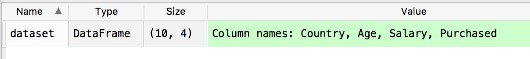
\includegraphics[scale=0.5]{figures/Chapter3AnnisaFathoroni7.jpeg}
\caption{Import Dataset}
\label{contoh}
\end{figure}

\item Lalu klik dataset cell, maka akan muncul seperti berikut :
\item Seperti yang terlihat pada gambar tersebut dataset ini memiliki Kolom Country, Age, dan Salary sebagai independent variable-nya dan kolom

\begin{figure}[ht]
\centering
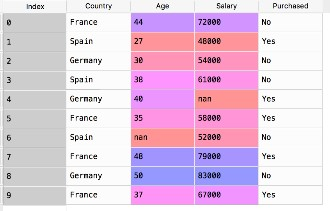
\includegraphics[scale=0.5]{figures/Chapter3AnnisaFathoroni8.jpeg}
\caption{Hasil Dataset Sel}
\label{contoh}
\end{figure}

\item Purchased sebagai dependent variable-nya.
\item Selanjutnya buat 2 matrix of features yang berisi values dari independent variable dan dependent variable.
\item Lalu tuliskan perintah berikut :

\begin{figure}[ht]
\centering
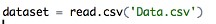
\includegraphics[scale=0.8]{figures/Chapter3AnnisaFathoroni9.jpeg}
\caption{Perintah}
\label{contoh}
\end{figure}

\item Perintah yang telah dibuat di atas akan membuat sebuah global environment baru dan muncul dataset.
\item Klik dataset tersebut maka muncul tabel berisi dataset.
\end{itemize}

\item Cross Validation

Cross-validation (CV) adalah metode statistik yang dapat digunakan untuk mengevaluasi kinerja model atau algoritma dimana data dipisahkan menjadi dua subset yaitu data proses pembelajaran dan data validasi / evaluasi. Model atau algoritma dilatih oleh subset pembelajaran dan divalidasi oleh subset validasi. Selanjutnya pemilihan jenis CV dapat didasarkan pada ukuran dataset. Biasanya CV K-fold digunakan karena dapat mengurangi waktu komputasi dengan tetap menjaga keakuratan estimasi.

\item Arti score 44\% pada random forest, 27\% pada decission tree dan 29\%dari SVM.

 Kalau maksud arti score 27\% pada decission tree adalah presentasi hasil dari perhitungan dataset, sedangkan maksud arti score 29\% dari SVM adalah hasil pendekatan jaringan saraf.  Hasil tersebut didapat dari hasil valdasi silang untuk memastikan bahwa membagi training test dengan cara yang berbeda. Sehingga didapat outputnya 44\% untuk hutan acak, 27\% untuk pohon keputusan, dan 29\% untuk SVM.

\item Confusion Matrix Dan Ilustrasinya
\begin{enumerate}
\item Perhitungan confusion matrix adalah sebagai berikut, akan saya beri contoh sederhana yaitu pengambilan keputusan untuk mendapatkan bantuan beasiswa. Saya menggunakan dua atribut, yaitu rekening listrik dan gaji. Ini adalah pohon keputusannya:
 
\begin{figure}[ht]
\centering
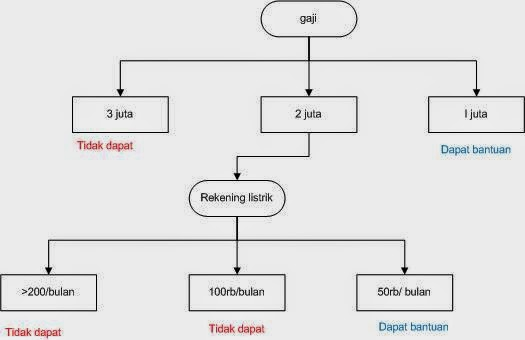
\includegraphics[scale=0.5]{figures/Chapter3AnnisaFathoroni2.jpg}
\caption{Pohon Keputusan}
\label{contoh}
\end{figure}
\end{enumerate}

Kemudian data testingnya adalah

\begin{figure}[ht]
\centering
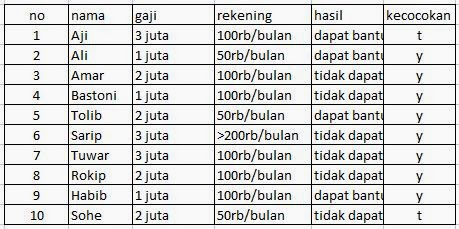
\includegraphics[scale=0.5]{figures/Chapter3AnnisaFathoroni3.jpg}
\caption{Data Testing}
\label{contoh}
\end{figure}

Yang pertama kita lakukan yaitu mencari 4 nilai yaitu a,b,c, dan d:

a= 5

b= 1

c= 1

d= 3

Kemudian kita dapat mencari nilai Recall, Precision, accuracy dan Error Rate

Recall =3/(1+3) = 0,75

Precision = 3/(1+3) = 0,75

Accuracy =(5+3)/(5+1+1+3) = 0,8

Error Rate =(1+1)/(5+1+1+3) = 0,2

\item Voting Random Forest Dan Ilustrasi Gambarnya.

\begin{itemize}
\item Pengertian Voting pada Random Forest

Metode ensemble dapat mencapai akurasi tinggi dengan membangun beberapa pengklasifikasi dan menjalankan masing-masing secara mandiri. Ketika classifier membuat keputusan, Anda dapat memanfaatkan yang terbaik keputusan umum dan rata-rata. Jika kita menggunakan metode yang paling umum, itu disebut voting

\item Ilustrasi Gambar Voting Random Forest :
\begin{figure}[ht]
\centering
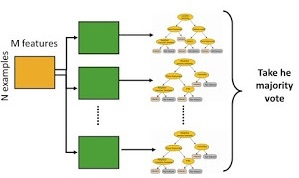
\includegraphics[scale=0.8]{figures/Chapter3AnnisaFathoroni4.jpg}
\caption{Voting Random Forest}
\label{contoh}
\end{figure}
\end{itemize}
\end{enumerate}

\section{Tasya Wiendhyra/1164086}
HARI PERTAMA TEORI
\section{Random Forest Dan Contohnya}
\subsection{Pengertian}
Random Forest adalah konstruk data yang diterapkan pada machine learning yang mengembangkan sejumlah besar pohon keputusan acak yang menganalisis sekumpulan variabel. Jenis algoritma ini membantu meningkatkan cara teknologi menganalisis data yang kompleks. Juga merupakan algoritma machine learning yang fleksibel, mudah digunakan, bahkan tanpa penyetelan hyper-parameter, dengan hasil yang baik. Ini juga merupakan salah satu algoritma yang paling banyak digunakan, karena kesederhanaan dan faktanya dapat digunakan untuk tugas klasifikasi dan regresi.\\
Dibawah ini merupakan salah satu ilustrasi penggunaan Random Forest yang saya lakukan untuk memprediksi apakah uang kertas bank otentik atau tidak berdasarkan pada empat atribut.
Ini merupakan hasil dari ilustrasi Random Forest pada Spyder
\begin{figure}[ht]
\centering
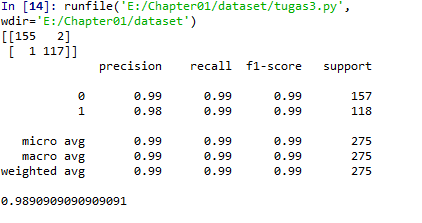
\includegraphics[scale=0.5]{figures/teori1.png}
\caption{Random Forest Spyder}
\label{Contoh}
\end{figure}
\par
Setelah di plotting hasilnya seperti berikut
\begin{figure}[ht]
\centering
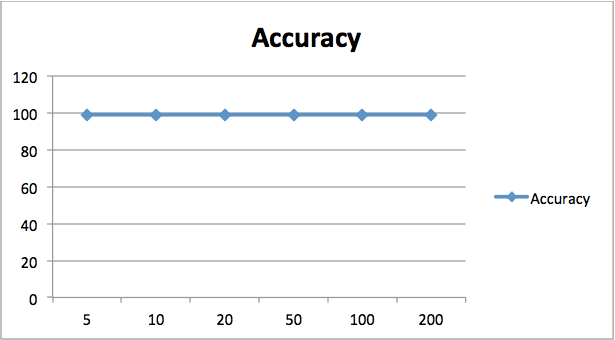
\includegraphics[scale=0.5]{figures/teori2.png}
\caption{Random Forest Graphic}
\label{Contoh}
\end{figure}

\section{Dataset}
\subsection{Pengertian Dataset}
Dataset adalah kumpulan data. Paling umum satu data set sesuai dengan isi tabel database tunggal, atau matriks data statistik tunggal, di mana setiap kolom tabel mewakili variabel tertentu, dan setiap baris sesuai dengan anggota tertentu dari dataset yang dipertanyakan.
\subsection{Cara Membaca Dataset Dan Arti Setiap File Dan Isi Field Masing Masing File}
\begin{enumerate}
\item
Gunakan librari Pandas pada python untuk dapat membaca dataset dengan format text file.
\item
Setelah itu, buat variabel baru "dataset" yang berisikan perintah untuk membaca file csv. seperti berikut
\begin{figure}[ht]
\centering
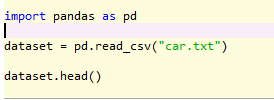
\includegraphics[scale=0.5]{figures/teori3.png}
\caption{Dataset Pandas}
\label{Contoh}
\end{figure}
\par
Pada gambar diatas dapat dijelaskan bahwa :\\
\begin{itemize}
\item
Memanggil Librari Panda untuk membaca dataset
\item
Membuat variabel "Dataset" yang berisikan pdreadcsv untuk membaca dataset. Pada contoh ini menggunakan txt tapi tetap bisa membaca datasetnya, mengapa? Karena pada saat dijalankan librari panda secara otomatis akan mengubah data dalam bentuk text file ke format csv.
\end{itemize}
\item
Setelah di run akan muncul hasil seperti berikut :
\begin{figure}[ht]
\centering
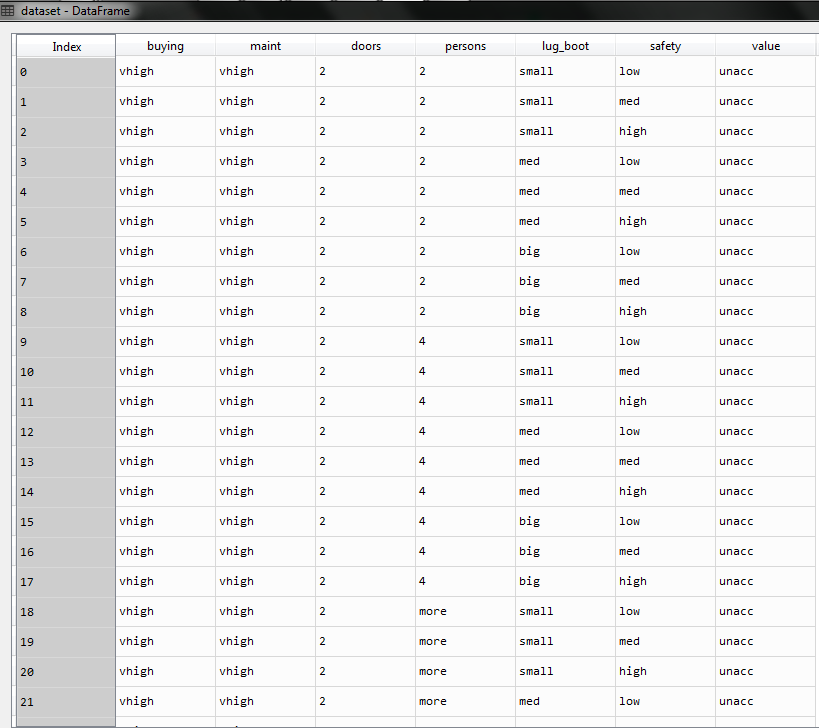
\includegraphics[scale=0.5]{figures/teori4.png}
\caption{Dataset Pandas}
\label{Contoh}
\end{figure}
\par
Pertama tama gambar diatas merupakan dataset yang digunakan untuk evaluasi mobil setelah dibuat untuk mengecek dan menguji induksi konstruktif dan metode penemuan struktur. Datasetnya dapat didapatkan dari laman https://archive.ics.uci.edu/ml/datasets/Car+Evaluation.\\
Penjelasan dari isi field diatas adalah sebagai berikut :\\
\begin{itemize}
\item
Atribut Index merupakan atribut otomatis untuk penomoran data yang ada.
\item
Atribut Buying merupakan harga beli dari mobil tersebut. dengan value : v high/Sangat mahal,high/mahal,med/Cukup, low/Murah.
\item
Atribut Maint merupakan harga perawatan dari mobil tersebut, dengan value sama seperti pada atribut Buying.
\item
Atribut Doors merupakan jumlah pintu yang terdapat pada mobil, dengan value 2,3,4,5 more atau lebih dari 5.
\item
Atribut Persons merupakan kapasitas orang yang bisa masuk kedapalm mobil, dengan value 2,4, more /lebih.
\item
Atribut Lug Boot merupakan ukuran bagasi boot mobil, dengan value small,med,big.
\item
Atribut Safety merupakan perkiraan keselamatan mobil, dengan value low,med,high.
\item
Yang terakhir yaitu Value, yang dimana merupakan merupakan Class nya atau disebut dengan targetnya menyatakan apakah mobil tersebut dapat diterima atau tidak dan apakah mobil tersebut bagus atau tidak, dengan value unacc, acc, good,v good .
\end{itemize}
\end{enumerate}

\section{Cross Validation}
Cross Validation adalah prosedur resampling yang digunakan untuk mengevaluasi model machine learning pada sampel data yang terbatas. Prosedur ini memiliki parameter tunggal yang disebut k yang mengacu pada jumlah grup tempat sampel data yang akan dibagi. Karena itu, prosedur ini sering disebut k-fold cross-validation.\\
Proses penentuan apakah hasil numerik yang mengukur hubungan yang dihipotesiskan antar variabel, dapat diterima sebagai deskripsi data, dikenal sebagai Validationi. Umumnya, estimasi kesalahan untuk model dibuat setelah training, lebih dikenal sebagai evaluasi residu. Dalam proses ini, estimasi numerik dari perbedaan respons yang diprediksi dan yang asli dilakukan, juga disebut kesalahan training. Namun, ini hanya memberi kita gambaran tentang seberapa baik model kita pada data yang digunakan untuk melatihnya. Sekarang mungkin bahwa model tersebut kurang cocok atau overfitting data. Jadi, masalah dengan teknik evaluasi ini adalah bahwa itu tidak memberikan indikasi seberapa baik pelajar akan menggeneralisasi ke set data independen / tidak terlihat. Model ini dikenal sebagai Cross Validation.

\section{Arti Score 44\% Pada Random Forest, 27\% Pada Decission Tree Dan 29\% Dari SVM}
Itu merupakan presentase keakurasian prediksi yang dilakukan pada saat testing menggunakan label pada dataset yang digunakan. Score merupakan mendefinisikan aturan evaluasi model. Maka pada saat dijalankan akan muncuk persentase tersebut yang menunjukan keakurasian atau keberhasilan dari prediksi yang dilakukan. Jika menggunakan Random Forest maka hasilnya 40\% , jika menggunakan Decission Tree hasil prediksinya yaitu 27\% dan pada SVM 29\% .

\section{Confusion Matriks}
\subsection{Confusion Matriks Dan Contohnya}
Perthitungan Confusion Matriks dapat dilakukan sebagai berikut. Disini saya menggunakan data yang dibuat sendiri untuk menampilkan data aktual dan prediksi.
\begin{itemize}
\item
Import librari Pandas, Matplotlib, dan Numpy.
\item
Buat variabel y actu yang berisikan data aktual.
\item
Buat variabel y pred berisikan data yang akan dijadikan sebagai prediksi.
\item
Buat variabel df confusion yang berisikan crosstab untuk membangun tabel tabulasi silang yang dapat menunjukkan frekuensi kemunculan kelompok data tertentu.
\item
Pada variabel df confusion definisikan lagi nama baris yaitu Actual dan kolomnya Predicted
\item
Kemudian definisikan suatu fungsi yang diberi nama plot confusion matrix yang berisikan pendefinisian confusion matrix dan juga akan di plotting. untuk code lengkapnya sebagai berikut 
\begin{verbatim}
import numpy as np
import matplotlib.pyplot as plt
import pandas as pd

y_actu = pd.Series([2, 0, 2, 2, 0, 1, 1, 2, 2, 0, 1, 2], name='Actual')
y_pred = pd.Series([0, 0, 2, 1, 0, 2, 1, 0, 2, 0, 2, 2], name='Predicted')
df_confusion = pd.crosstab(y_actu, y_pred)

df_confusion = pd.crosstab(y_actu, y_pred, rownames=['Actual'], colnames=['Predicted'], margins=True)

def plot_confusion_matrix(df_confusion, title='Confusion matrix', cmap=plt.cm.gray_r):
    plt.matshow(df_confusion, cmap=cmap) # imshow
    #plt.title(title)
    plt.colorbar()
    tick_marks = np.arange(len(df_confusion.columns))
    plt.xticks(tick_marks, df_confusion.columns, rotation=45)
    plt.yticks(tick_marks, df_confusion.index)
    #plt.tight_layout()
    plt.ylabel(df_confusion.index.name)
    plt.xlabel(df_confusion.columns.name)

plot_confusion_matrix(df_confusion)

plt.show()
\end{verbatim}

\par

Hasilnya akan seperti berikut :
\begin{figure}[ht]
\centering
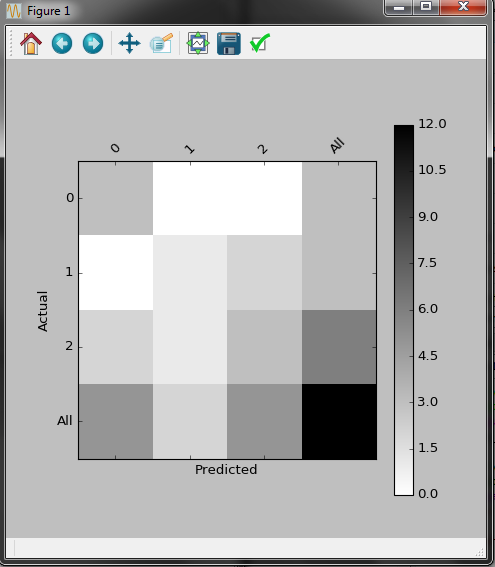
\includegraphics[scale=0.5]{figures/teori5.png}
\caption{Confusion Matrix}
\label{Contoh}
\end{figure}
\end{itemize}

\section{Voting Pada Random Forest}
\subsection{Pengertian}
Voting yaitu suara untuk setiap target yang diprediksi pada saat melakukan Random Forest. Pertimbangkan target prediksi dengan voting tertinggi sebagai prediksi akhir dari algoritma random forest.
\subsection{Contoh}
\begin{itemize}
\item
Untuk menggunakan Voting pada Random Forest dapat dilihat code berikut. Disini saya mengilustrasikan voting untuk berbagai macam algoritma terutama Random Forest.
\begin{verbatim}
import numpy as np
import matplotlib.pyplot as plt

from sklearn.linear_model import LogisticRegression
from sklearn.naive_bayes import GaussianNB
from sklearn.ensemble import RandomForestClassifier
from sklearn.ensemble import VotingClassifier

clf1 = LogisticRegression(solver='lbfgs', max_iter=1000, random_state=123)
clf2 = RandomForestClassifier(n_estimators=100, random_state=123)
clf3 = GaussianNB()
X = np.array([[-1.0, -1.0], [-1.2, -1.4], [-3.4, -2.2], [1.1, 1.2]])
y = np.array([1, 1, 2, 2])

eclf = VotingClassifier(estimators=[('lr', clf1), ('rf', clf2), ('gnb', clf3)],
                        voting='soft',
                        weights=[1, 1, 5])

# predict class probabilities for all classifiers
probas = [c.fit(X, y).predict_proba(X) for c in (clf1, clf2, clf3, eclf)]

# get class probabilities for the first sample in the dataset
class1_1 = [pr[0, 0] for pr in probas]
class2_1 = [pr[0, 1] for pr in probas]


# plotting

N = 4  # number of groups
ind = np.arange(N)  # group positions
width = 0.35  # bar width

fig, ax = plt.subplots()

# bars for classifier 1-3
p1 = ax.bar(ind, np.hstack(([class1_1[:-1], [0]])), width,
            color='green', edgecolor='k')
p2 = ax.bar(ind + width, np.hstack(([class2_1[:-1], [0]])), width,
            color='lightgreen', edgecolor='k')

# bars for VotingClassifier
p3 = ax.bar(ind, [0, 0, 0, class1_1[-1]], width,
            color='blue', edgecolor='k')
p4 = ax.bar(ind + width, [0, 0, 0, class2_1[-1]], width,
            color='steelblue', edgecolor='k')

# plot annotations
plt.axvline(2.8, color='k', linestyle='dashed')
ax.set_xticks(ind + width)
ax.set_xticklabels(['LogisticRegression\nweight 1',
                    'GaussianNB\nweight 1',
                    'RandomForestClassifier\nweight 5',
                    'VotingClassifier\n(average probabilities)'],
                   rotation=40,
                   ha='right')
plt.ylim([0, 1])
plt.title('Class probabilities for sample 1 by different classifiers')
plt.legend([p1[0], p2[0]], ['class 1', 'class 2'], loc='upper left')
plt.tight_layout()
plt.show()
\end{verbatim}
\item
Hasilnya sebagai berikut 
\begin{figure}[ht]
\centering
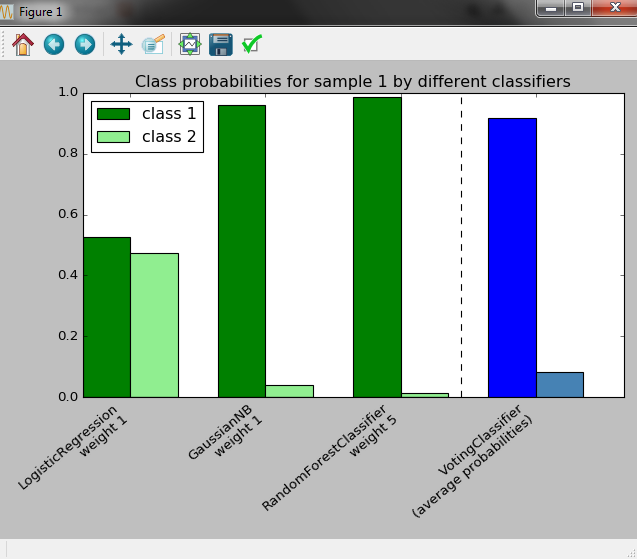
\includegraphics[scale=0.5]{figures/teori6.png}
\caption{Voting Random Forest}
\label{Contoh}
\end{figure}
\end{itemize}

\section{Annisa Cahyani/1164066}
\subsection{Teori}
Penyelesaian Tugas Harian 5 ( No. 1-6 )
\begin{enumerate}
\item Random Forest Dan Ilustrasi Gambarnya
\begin{itemize}
\item Pengertian Random Forest:
\par Random forest (RF) adalah suatu algoritma yang digunakan pada klasifikasi data dalam jumlah yang besar. Klasifikasi random forest dilakukan melalui penggabungan pohon (tree) dengan melakukan training pada sampel data yang dimiliki. Penggunaan pohon (tree) yang semakin banyak akan mempengaruhi akurasi yang akan didapatkan menjadi lebih baik. Penentuan klasifikasi dengan random forest diambil berdasarkan hasil voting dari tree yang terbentuk.
\end{itemize}
\item Cara Membaca Dataset, Dan artikan makna setiap file dan isinya.
\end{enumerate}
\begin{itemize}
\item Cara Membaca Dataset :
\end{itemize}
\par Membaca Dataset
\begin{enumerate}
\item Langkah-langkah  yang harus di lakukan yaitu:
\begin{itemize}
\item Pertama kita harus membuka Aplikasi yang digunakan untuk membuka datasetnya terlebih dahulu 
\item saya menggunakan spyder dari Anaconda Navigator
\item kemudian kita import libraries seperti numphy, pandas, matplotlib dll ( sesuai yang dibutuhkan ).
\item lalu untuk memasukkan kode python yang akan digunakan untuk membaca file csv yang berada pada dataset 
\end{itemize}
\item Cross Validation Dan Ilustrasi Gambar :
\begin{itemize}
\item Pengertian Cross Validation :
\par Cross Validation merupakan salah satu dari berbagai teknik validasi untuk menilai bagaimana hasil analisis statistik yang akan digeneralisasikan ke set data independen. Biasanya yang digunakan dalam pengaturan itu tujuannya  untuk memprediksi, dan  memperkirakan seberapa akurat model prediksi yang akan dilakukan dalam praktek. 
\par 
\end{itemize}
\par
\item Penjelasan / Maksud Dari Score pada :
\begin{itemize}
\item Random forest ( 44 \% )
\par 
\par
\item Decision Tree ( 27 \% )
\par 
\par
\item SVM ( 29 \% )
\end{itemize}
\item Confusion Matrix Dan Ilustrasinya :
\begin{itemize}
\item Pengertian Confusion Matrix :
\par Confusion matrix merupakan salah satu metode yang dapat digunakan untuk mengukur kinerja suatu metode klasifikasi. Pada dasarnya confusion matrix mengandung informasi yang membandingkan hasil klasifikasi yang dilakukan oleh sistem dengan hasil klasifikasi yang seharusnya.
\item Cara Membaca Confusion Matrix :
\par Untuk cara pembacaan dan pemahaman pada confusion matrix sebagai berikut :
\item Ketika hasil prediksinya itu negatif dan data sebenarnya merupakan negatif.
\item Ketika hasil prediksinya itu positif sedangkan nilai sebenarnya merupakan negatif.
\item Ketika hasil prediksinya itu negatif sedangkan nilai sebenarnya merupakan positif.
\item Ketika hasil prediksinya itu positif dan nilai sebenarnya merupakan positif.
\end{itemize}
\par

\par
\par
\item Voting Random Forest Dan Ilustrasi Gambarnya.
\par
\begin{itemize}
\item Pengertian Voting pada Random Forest :
\par Voting pada random forest yaitu suatu penetuan hasil klasifikasi yang akan diambil atau hasil dari hasil pengklasifikasian data
\par 
\end{itemize}
\end{enumerate}

\section{Praktek Program}
\section{Tasya Wiendhyra / 1164086}
HARI KEDUA PRAKTEK MINGGU KETIGA
\subsection{Aplikasi Sederhana Menggunakan Pandas}
Disini saya akan membuat program sederhana menggunakan Pandas yaitu untuk memilih baris dari DataFrame yang diberikan berdasarkan value di salah satu kolom.
\begin{lstlisting}[caption=Code Program Sederhana Pandas,label={lst:3.1}]
import pandas as pd
d = {'kol1': [1, 4, 3, 4, 5], 'kol2': [4, 5, 6, 7, 8], 'kol3': [7, 8, 9, 0, 1]}
df = pd.DataFrame(data=d)
print("Original DataFrame")
print(df)
print('Baris Untuk kolom2 dengan value 7')
print(df.loc[df['kol2'] == 7 ] )
\end{lstlisting}
Dari code diatas dapat dijelaskan perbarisnya sebagai berikut :\\
\begin{itemize}
\item
Baris pertama, yaitu import pandas yang artinya kita akan mengimport librari Pandas dari python dengan inisiasi pd.
\item
Variabel d didefinisikan data data untuk kolom 1, kolom2, dan kolom3 
\item
Variabel df akan mengubah data pada variabel d disejajarkan menjadi baris dan kolom dengan menggunakan pd dataframe.
\item
Baris selanjutnya yaitu akan mencetak atau menampilkan tulisan Original dataFrame pada jendela konsol.
\item
Print df artinya akan mencetak atau menampilkan DataFrame dari data yang telah dibuat tadi.
\item
Baris selanjutnya yaitu akan mencetak atau menampilkan tulisan Baris Untuk kolom2 dengan value 7 pada jendela konsol.
\item
Baris terakhir akan menampilkan data yang telah disortir berdasarkan perintah. Dimana hanya akan menampilkan data yang terdapat value 7 pada kolom 2.
\end{itemize}

Hasilnya sebagai berikut :
\begin{figure}[ht]
\centering
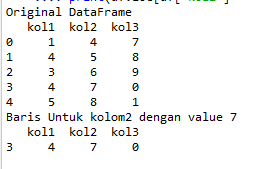
\includegraphics[scale=0.5]{figures/praktek1.png}
\caption{Aplikasi Sederhana Menggunakan Pandas}
\label{Praktek}
\end{figure}

\subsection{ Aplikasi Sederhana Menggunakan Numpy}
Program yang akan dibuat yaitu menentukan atau menemukan  nilai yang sama dari dua array . dapat dilihat dalam lsting \ref{lst:3.2}.
\begin{lstlisting}[caption=Code Program Sederhana Numpy,label={lst:3.2}]
import numpy as np
array1 = np.array([0, 10, 20, 40, 60])
print("Array1: ",array1)
array2 = np.array([10, 30, 40])
print("Array2: ",array2)
print("Data Yang Sama Dari Kedua Array Adalah:")
print(np.intersect1d(array1, array2))
\end{lstlisting}

Dari code diatas dapat dijelaskan perbarisnya sebagai berikut :\\
\begin{itemize}
\item
Baris pertama, yaitu import numpy yang artinya kita akan mengimport librari Numpy dari python dengan inisiasi np.
\item
Variabel array1 berisikan np array yang dimana akan membuat sebuah Array berisikan value yang telah disebutkan.
\item
Akan mencetak tulisan "Array1" dan menampilkan data dari variabel array1.
\item
Variabel array2 berisikan np array yang dimana akan membuat sebuah Array berisikan value yang telah disebutkan.
\item
Akan mencetak tulisan "Array2" dan menampilkan data dari variabel array2.
\item
Baris selanjutnya akan mencetak dan menampilkan tulisan "Data Yang Sama Dari Kedua Array Adalah:" pada jendela konsol.
\item
Dan yang terakhir np intersect1d akan menampilkan irisan dari array1 dan array2
\end{itemize}

Hasilnya sebagai berikut :
\begin{figure}[ht]
\centering
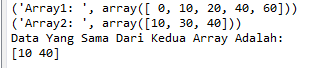
\includegraphics[scale=0.5]{figures/praktek2.png}
\caption{Aplikasi Sederhana Menggunakan Numpy}
\label{Praktek}
\end{figure}
\subsection{Aplikasi Sederhana Menggunakan Matplotlib}
Program yang akan dibuat yaitu membuat dua baris atau lebih dengan lebar dan warna yang berbeda. Code lengkap pada lsting \ref{lst:3.3}
\begin{lstlisting}[caption=Code Program Sederhana Matplotlib,label={lst:3.3}]
import matplotlib.pyplot as plt
# line 1 points
x1 = [10,20,30]
y1 = [20,40,10]
# line 2 points
x2 = [10,20,30]
y2 = [40,10,30]
# Set the x axis label of the current axis.
plt.xlabel('x - Cintaku')
# Set the y axis label of the current axis.
plt.ylabel('y - Cintamu')
# Set a title 
plt.title('Dua Baris Atau Lebih Dengan Lebar Dan Warna Yang Berbeda Guys ')
# Display the figure.
plt.plot(x1,y1, color='salmon', linewidth = 3,  label = 'line1 lebar 3')
plt.plot(x2,y2, color='mediumvioletred', linewidth = 5,  label = 'line2 lebar 5')
# show a legend on the plot
plt.legend()
plt.show()
\end{lstlisting}
Dari code diatas dapat dijelaskan sebagai berikut :\\
\begin{itemize}
\item
Pertama tama yaitu akan meng import librari Pyplot dari  Matplotlib sebagai plt.
\item
Variabel x1 dan y1 akan berisikan value untuk titik atau point dari garis 1 nya.
\item
Begitu juga dengan variabel x2 dan y2 akan berisikan value untuk titik atau point dari garis 2 nya.
\item
Plt.xlabel akan mengatur label sumbu x dari axis saat ini dengan nama x Cintaku.
\item
Plt.ylabel akan mengatur label sumbu y dari axis saat ini dengan nama x Cintamu.
\item
Plt title akan mendefinisikan title atau judul dari grafik ini.
\item
plt plot akan menampilkan figurenya. Untuk line 1 diberi warna salmon dengan lebar garisnya 3 cm diberi label "line1 lebar 3". Dan untuk  line 2 diberi warna mediumvioletred dengan lebar garisnya 5 cm diberi label "line2 lebar 5".
\item
plt legend untuk menampilkan legend 
\item
Plt show digunakan untuk menampilkan grafik pada saat skrip dijalankan.
\end{itemize}

Hasilnya sebagai berikut :
\begin{figure}[ht]
\centering
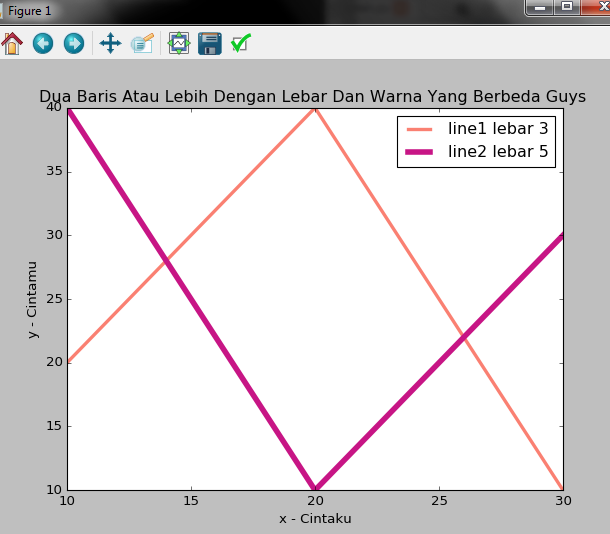
\includegraphics[scale=0.3]{figures/praktek3.png}
\caption{Aplikasi Sederhana Menggunakan Matplotlib}
\label{Praktek}
\end{figure}
\subsection{Menjalankan Program Klasifikasi Random Forest}
Berikut adalah output dari percobaan Random Forest yang telah dilakukan
\begin{itemize}
\item Jika dilihat dari outputnya, code berikut berfungsi untuk membaca data yang berupa dataset dengan format text file. Dengan mendefinisikan variabel imgatt yang berisikan value untuk membaca data, juga menggunakan code untuk skip data yang mengandung bad lines agar tidak terjadi eror pada saat pembacaan file.
\begin{figure}[ht]
\centering
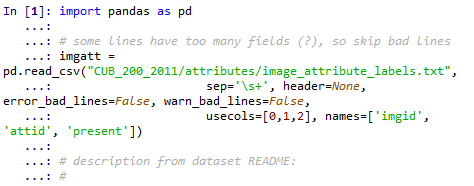
\includegraphics[scale=0.5]{figures/rf1.png}\newpage
\caption{Program Random Forest Tasya}
\label{Praktek}
\end{figure}
\item Output ini mengembalikan baris n teratas (5 secara default) dari dataframe imgatt.
\begin{figure}[ht]
\centering
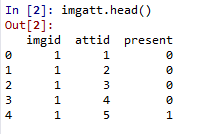
\includegraphics[scale=0.5]{figures/rf2.png}
\caption{Program Random Forest Tasya}
\label{Praktek}
\end{figure}
\\
\item Output ini menampilkan jumlah baris dan kolom dari dataframe imgatt.
\begin{figure}[ht]
\centering
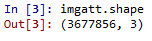
\includegraphics[scale=0.5]{figures/rf3.png}
\caption{Program Random Forest Tasya}
\label{Praktek}
\end{figure}
\\
\item Dari outputnya dapat dilihat bahwa variabel imgatt2 menggunakan function pivot untuk mengubah kolom jadi baris, dan baris jadi kolom dari dataframe sebelumnya.
\begin{figure}[ht]
\centering
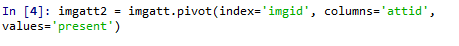
\includegraphics[scale=0.5]{figures/rf4.png}
\caption{Program Random Forest Tasya}
\label{Praktek}
\end{figure}
\\
\\
\item Sama seperti output sebelumnya, imgatt2 head itu berfungsi untuk mengembalikan nilai atau value teratas dari dataframe imgatt2.
\begin{figure}[ht]
\centering
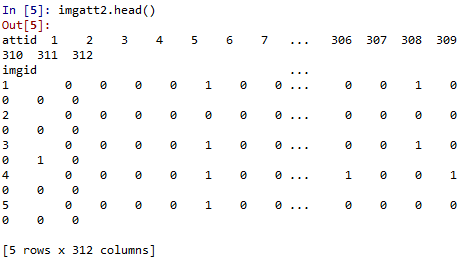
\includegraphics[scale=0.5]{figures/rf5.png}
\caption{Program Random Forest Tasya}
\label{Praktek}
\end{figure}
\\
\\
\\
\\
\item Output ini menampilkan jumlah baris dan kolom dari dataframe imgatt2
\begin{figure}[ht]
\centering
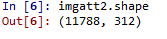
\includegraphics[scale=0.5]{figures/rf6.png}
\caption{Program Random Forest Tasya}
\label{Praktek}
\end{figure}
\item Dan melakukan pivot yang mana imgid menjadi index yang artinya unik.
\begin{figure}[ht]
\centering
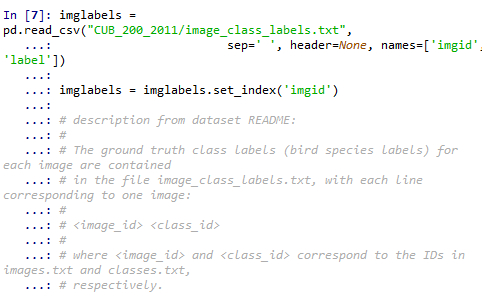
\includegraphics[scale=0.3]{figures/rf7.png}
\caption{Program Random Forest Tasya}
\label{Praktek}
\end{figure}
\\
\\
\\
\\
\\
\\
\\
\\
\\
\\
\item Output diatas akan meload jawabannya yang berisi apakah burung itu termasuk dalam spesies yang mana. Dua kolomnya adalah imgid dan label.
\begin{figure}[ht]
\centering
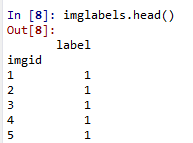
\includegraphics[scale=0.5]{figures/rf8.png}
\caption{Program Random Forest Tasya}
\label{Praktek}
\end{figure}
\item Output dari percobaan sebelumnya, menunjukkan 11788 baris dan 1 kolom. Dimana kolom itu adalah jenis spesies burungnya.
\begin{figure}[ht]
\centering
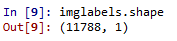
\includegraphics[scale=0.5]{figures/rf9.png}
\caption{Program Random Forest Tasya}
\label{Praktek}
\end{figure}
\item Melakukan join antara imgatt2 dengan imglabels karena isinya sama. Sehingga kita akan mendapatkan data ciri dan data jawabannya atau labelnya sehingga bisa dikatekorikan supervised learning.
\begin{figure}[ht]
\centering
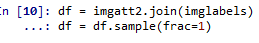
\includegraphics[scale=0.5]{figures/rf10.png}
\caption{Program Random Forest Tasya}
\label{Praktek}
\end{figure}
\item Output diatas akan drop label yang didepan, dan menggunakan label yang paling belakang yang baru di join.
\begin{figure}[ht]
\centering
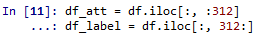
\includegraphics[scale=0.5]{figures/rf11.png}
\caption{Program Random Forest Tasya}
\label{Praktek}
\end{figure}
\item Output berikut mengecek isinya. Ini mengecek 5 data teratas dari df att
\begin{figure}[ht]
\centering
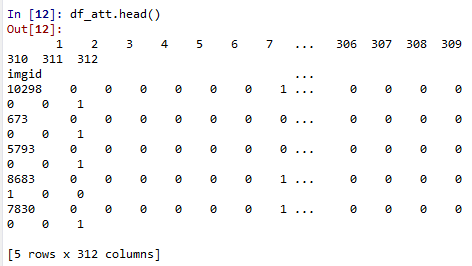
\includegraphics[scale=0.5]{figures/rf12.png}
\caption{Program Random Forest Tasya}
\label{Praktek}
\end{figure}
\item Output berikut mengecek isinya. Ini mengecek 5 data teratas dari df label
\begin{figure}[ht]
\centering
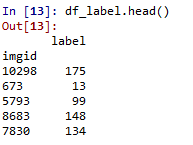
\includegraphics[scale=0.5]{figures/rf13.png}
\caption{Program Random Forest Tasya}
\label{Praktek}
\end{figure}
\item Output diatas membagi menjadi dua bagian, 8000 row pertama sebagai data training sisanya sebagai data testing.
\begin{figure}[ht]
\centering
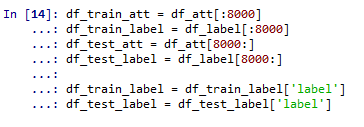
\includegraphics[scale=0.5]{figures/rf14.png}
\caption{Program Random Forest Tasya}
\label{Praktek}
\end{figure}
\item Memanggil kelas RandomForestClassifier. max features diartikan sebagai berapa banyak kolom pada setiap tree disini kolom pada setiap tree adalah 50.
\begin{figure}[ht]
\centering
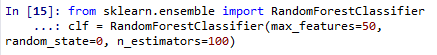
\includegraphics[scale=0.5]{figures/rf15.png}
\caption{Program Random Forest Tasya}
\label{Praktek}
\end{figure}
\item Output ini melakukan fit untuk membangun random forest yang sudah ditentukan dengan maksimum fitur sebanya 50 untuk perpohonnya.
\begin{figure}[ht]
\centering
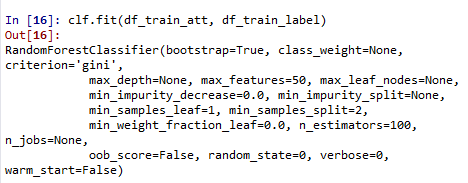
\includegraphics[scale=0.5]{figures/rf16.png}
\caption{Program Random Forest Tasya}
\label{Praktek}
\end{figure}
\item Menampilkan hasil prediksi dari random forest sebelumnya.
\begin{figure}[ht]
\centering
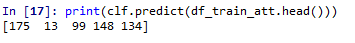
\includegraphics[scale=0.5]{figures/rf17.png}
\caption{Program Random Forest Tasya}
\label{Praktek}
\end{figure}
\item Menampilkan besaran akurasinya dari prediksi diatas atau Score perolehan dari klasifikasi.
\begin{figure}[ht]
\centering
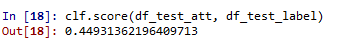
\includegraphics[scale=0.5]{figures/rf18.png}
\caption{Program Random Forest Tasya}
\label{Praktek}
\end{figure}
\end{itemize}

\subsection{Menjalankan Program Confusion Matrix}
Berikut adalah output dari percobaan Confusion Matrix yang telah dilakukan
\begin{itemize}
\item  Memetakan Random Forest ke dalam Confusion Matrix
\begin{figure}[ht]
\centering
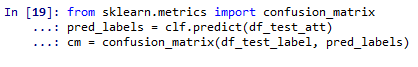
\includegraphics[scale=0.5]{figures/cm1.png}
\caption{Program Confusion Matrix Tasya}
\label{Praktek}
\end{figure} 

\item  Melihat hasil dari gambar diatas
\begin{figure}[ht]
\centering
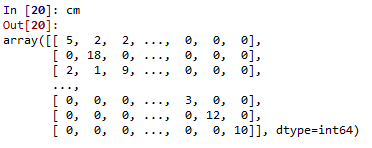
\includegraphics[scale=0.5]{figures/cm2.png}
\caption{Program Confusion Matrix Tasya}
\label{Praktek}
\end{figure} 

\item Plotting Confusion Matrix dengan Matplotlib
\begin{figure}[ht]
\centering
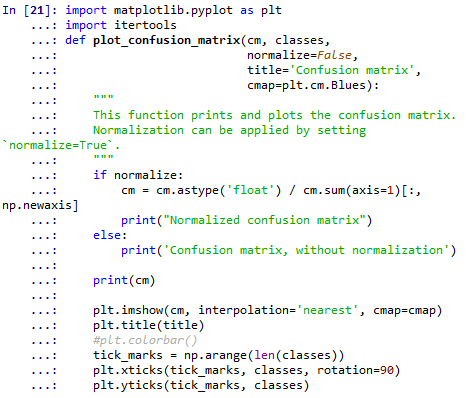
\includegraphics[scale=0.5]{figures/cm3.png}
\caption{Program Confusion Matrix Tasya}
\label{Praktek}
\end{figure}

\item Set plot sumbunya sesuai dengan nama datanya dan membaca file classes txt
\begin{figure}[ht]
\centering
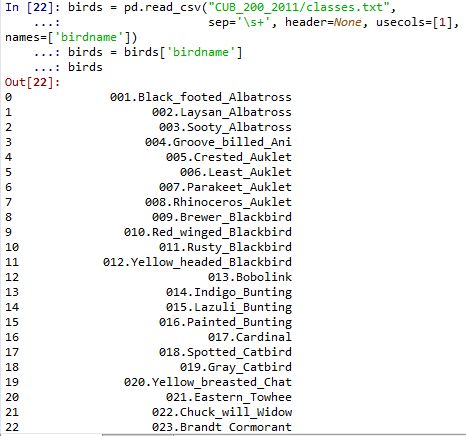
\includegraphics[scale=0.5]{figures/cm4.png}
\caption{Program Confusion Matrix Tasya}
\label{Praktek}
\end{figure}

\item Plot hasil perubahan label
\begin{figure}[ht]
\centering
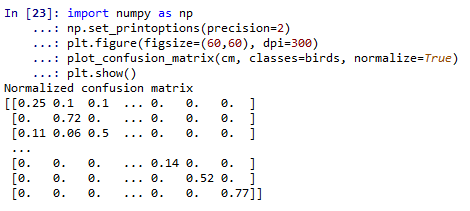
\includegraphics[scale=0.5]{figures/cm5.png}
\caption{Program Confusion Matrix Tasya}
\label{Praktek}
\end{figure}
\end{itemize}

\subsection{Menjalankan Program  Klasifikasi SVM dan Decission Tree}
Berikut adalah output dari percobaan  Klasifikasi SVM dan Decission Tree yang telah dilakukan
\begin{itemize}
\item Mencoba klasifikasi dengan decission tree dengan dataset yang sama dan akan muncul akurasi prediksinya.
\begin{figure}[ht]
\centering
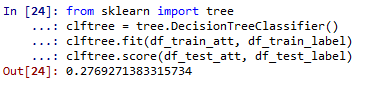
\includegraphics[scale=0.5]{figures/tree1.png}
\caption{Program Decission Tree Tasya}
\label{Praktek}
\end{figure}

\item Mencoba klasifikasi dengan SVM dengan dataset yang sama dan akan muncul akurasi prediksinya.
\begin{figure}[ht]
\centering
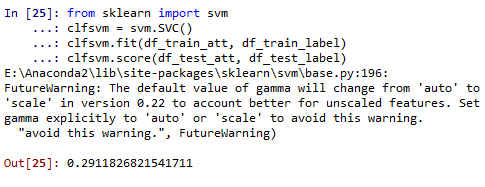
\includegraphics[scale=0.5]{figures/svm1.png}
\caption{Program SVM Tasya}
\label{Praktek}
\end{figure}
\end{itemize}

\subsection{Menjalankan Program Cross Validation}
Berikut adalah output dari percobaan  Cross Validation yang telah dilakukan
\begin{itemize}
\item Hasil Cross Validation untuk  Random Forest
\begin{figure}[ht]
\centering
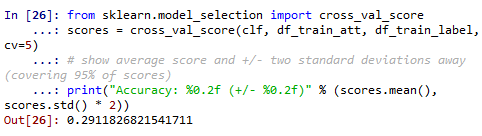
\includegraphics[scale=0.5]{figures/cv1.png}
\caption{Program Cross Validation Tasya}
\label{Praktek}
\end{figure}

\item Hasil Cross Validation untuk Decission Tree
\begin{figure}[ht]
\centering
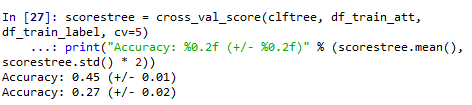
\includegraphics[scale=0.5]{figures/cv2.png}
\caption{Program Cross Validation Tasya}
\label{Praktek}
\end{figure}

\item Hasil Cross Validation untuk SVM
\begin{figure}[ht]
\centering
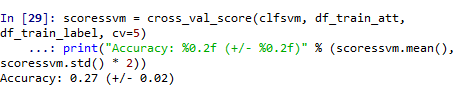
\includegraphics[scale=0.5]{figures/cv3.png}
\caption{Program Cross Validation Tasya}
\label{Praktek}
\end{figure}
\end{itemize}

\subsection{Menjalankan Program Komponen Informasi}
Berikut adalah output dari percobaan Komponen Informasi yang telah dilakukan
\begin{itemize}
\item Dari output ini dapat mengetahui berapa banyak tree yang dibuat, berapa banyak atribut yang dipakai dan informasi lainnya
\begin{figure}[ht]
\centering
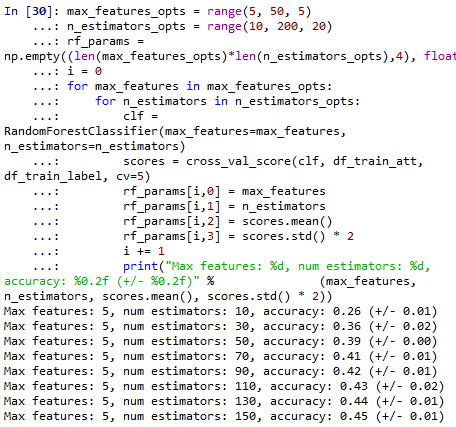
\includegraphics[scale=0.5]{figures/ki1.png}
\caption{Program Komponen Informasi Tasya}
\label{Praktek}
\end{figure}

\item Output berikut merupakan hasil dari plotting komponen informasi agar dapat dibaca
\begin{figure}[ht]
\centering
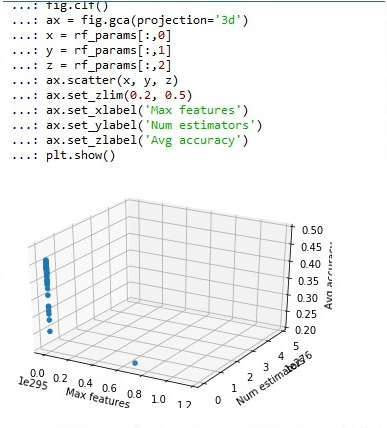
\includegraphics[scale=0.5]{figures/ki2.png}
\caption{Program Komponen Informasi Tasya}
\label{Praktek}
\end{figure}
\end{itemize}

\section{Penanganan Error}
HARI KEDUA TASYA WIENDHYRA 1164086
\subsection{Error Index}
\begin{enumerate}
	\item
Berikut ini merupakan eror yang didapatkan saat menjalankan program diatas
\begin{figure}[ht]
\centering
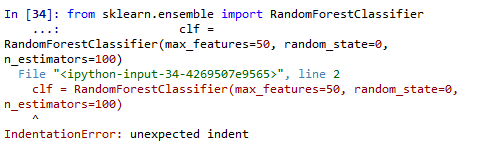
\includegraphics[scale=0.5]{figures/eror3.png}
\caption{Error Index}
\label{Error}
\end{figure}
	\item
Pada gambar diatas kode erornya adalah IndentationError unexpected indent. Eror ini terjadi karena adanya inkosisten pemberian indent di kode program.
	\item
Solusi yang bisa dilakukan untuk mengatasi eror tersebut adalah sebagai berikut : 
\end{enumerate}
\begin{itemize}
\item
Buka file code program dan lihat pada bagian erornya
\begin{figure}[ht]
\centering
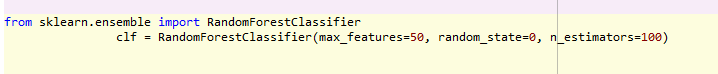
\includegraphics[scale=0.5]{figures/solusi9.png}
\caption{File Codingan}
\label{Eror}
\end{figure}
\item
Dapat dilihat pada baris kedua terdapat spasi dibagian depan, hilangkan atau hapus spasi tersebut seperti berikut 
\begin{figure}[ht]
\centering
\includegraphics[scale=0.5]{figures/solusi10.png}
\caption{Menghapus Spasi}
\label{Eror}
\end{figure}
\item Save, kemudian ketika dijalankan eror akan teratasi
\begin{figure}[ht]
\centering
\includegraphics[scale=0.5]{figures/solusi11.png}
\caption{Eror Teratasi}
\label{Eror}
\end{figure}
\end{itemize}

\subsection{ANNISA FATHORONI/1164067}
Penyelesaian Tugas Harian 6 ( No. 1-8 )
\begin{enumerate}
\item Aplikasi Sederhana Pandas dan Penjelasan Code
\begin{itemize}
\item Code Pandas:

\begin{verbatim}
import pandas as pd
d1 = {'a': 100, 'b': 200, 'c':300, 'd':400, 'e':800}
print("Original dictionary:")
print(d1)
new_series = pd.Series(d1)
print("Converted series:")
print(new_series)
\end{verbatim}

\begin{itemize}
\item Penjelasan Code Baris 1 : Memasukkan modul pandas sebagai variabel pd.

\item Penjelasan Code Baris 2 : Besaran nilai a, b , c, d dan e.

\item Penjelasan Code Baris 3 : Output atau keluaran bacaan 'Original Dictionary'

\item Penjelasan Code Baris 4 : Nilai dari D1 dikeluarkan.

\item Penjelasan Code Baris 5 : Membuat series baru dengan patokan nilai dari variabel d1.

\item Penjelasan Code Baris 6 : Mengeluarkan atau output dari Converted series.

\item Penjelasan Code Baris 7 : Mengeluarkan atau output dari series baru yang telah dibuatkan.

\end{itemize}
\item Hasil Eksekusi :

\begin{figure}[ht]
\centering
\includegraphics[scale=0.6]{figures/Chapter3AnnisaFathoroniPandas2.jpg}
\caption{Hasil Pandas/Annisa Fathoroni}
\label{contoh}
\end{figure}

\end{itemize}

\item Aplikasi Sederhana Numpy dan Penjelasan Code.
\begin{itemize}
\item Code Numpy:
 
\begin{verbatim}
import numpy as np
x = np.arange(12, 38)
print(x)
\end{verbatim}

\begin{itemize}
\item Penjelasan Code Baris 1 : Memasukkan modul numpy sebagai variabel np.

\item Penjelasan Code Baris 2 : Nilai antara angka 12-38.

\item Penjelasan Code Baris 3 :Mengeluarkan atau output dari proses.

\end{itemize}
\item Hasil Eksekusi :

\begin{figure}[ht]
\centering
\includegraphics[scale=0.6]{figures/Chapter3AnnisaFathoroniNumpy2.jpg}
\caption{Hasil Numpy/Annisa Fathoroni}
\label{contoh}
\end{figure}

\end{itemize}

\item Aplikasi Sederhana Matplotlib dan Penjelasan Code.
\begin{itemize}
\item Code Matplotlib:

\begin{verbatim}
import matplotlib.pyplot as plt
X = range(1, 50)
Y = [value * 3 for value in X]
plt.plot(X, Y)
plt.xlabel('x - axis')
plt.ylabel('y - axis')
plt.title('Draw a line.')
print(plt.axis()) 
plt.axis([0, 100, 0, 200]) 
plt.show()
\end{verbatim}

\begin{itemize}
\item Penjelasan Code Baris 1 : Memasukkan modul Matplotlib sebagai variabel plt

\item Penjelasan Code Baris 2 : Nilai X dengan ukuran 1-50.

\item Penjelasan Code Baris 3 : Nilai Y dikalikan 3 untuk menjadi nilai di dalam X

\item Penjelasan Code Baris 4 : Matplotlib dengan koordinat X dan Y

\item Penjelasan Code Baris 5 : Judul  atau keterangan label X

\item Penjelasan Code Baris 6 : Judul atau keterangan label Y

\item Penjelasan Code Baris 7 : Judul atau keterangan Diatas.

\item Penjelasan Code Baris 8 : Print, mengeluarkan atau output.

\item Penjelasan Code Baris 9 : Nilai plt antara 0-200.

\item Penjelasan Code Baris 10 : Menampilkan matplotlib
\end{itemize}
\item Hasil Eksekusi :


\begin{figure}[ht]
\centering
\includegraphics[scale=0.6]{figures/Chapter3AnnisaFathoroniMatplotlib2.jpg}
\caption{Hasil Matplotlib/Annisa Fathoroni}
\label{contoh}
\end{figure}

\end{itemize}

\item Program Aplikasi Random Forest dan Penjelasan Keluarannya.
\begin{itemize}
\item Code Random Forest 1:

\begin{figure}[ht]
\centering
\includegraphics[scale=0.6]{figures/Chapter3AnnisaFathoroni10.jpg}
\caption{Random Forest 1/Annisa Fathoroni}
\label{contoh}
\end{figure}

\begin{itemize}
\item Penjelasan :

Membaca dataset file txt.
 
\end{itemize}
\item Code Random Forest 2:

\begin{figure}[ht]
\centering
\includegraphics[scale=0.6]{figures/Chapter3AnnisaFathoroni11.jpg}
\caption{Random Forest 2/Annisa Fathoroni}
\label{contoh}
\end{figure}

\begin{itemize}
\item Penjelasan :

Melihat sebagian data awal, dengan menggunakan listing.

\end{itemize}
\item Code Random Forest 3:

\begin{figure}[ht]
\centering
\includegraphics[scale=0.6]{figures/Chapter3AnnisaFathoroni12.jpg}
\caption{Random Forest 3/Annisa Fathoroni}
\label{contoh}
\end{figure}

\begin{itemize}
\item Penjelasan :

Melihat jumlah data menggunakan listing.

\end{itemize}
\item Code Random Forest 4:

\begin{figure}[ht]
\centering
\includegraphics[scale=0.6]{figures/Chapter3AnnisaFathoroni13.jpg}
\caption{Random Forest 4/Annisa Fathoroni}
\label{contoh}
\end{figure}

\begin{itemize}
\item Penjelasan :

Privot dataset.

\end{itemize}
\item Code Random Forest 5:

\begin{figure}[ht]
\centering
\includegraphics[scale=0.6]{figures/Chapter3AnnisaFathoroni14.jpg}
\caption{Random Forest 5/Annisa Fathoroni}
\label{contoh}
\end{figure}

\begin{itemize}
\item Penjelasan :

Mengubah atribut menjadi kolom dengan menggunakan ptivot layaknya excel, lalu cek isi menggunakan perintah pada listing.

\end{itemize}
\item Code Random Forest 6:

\begin{figure}[ht]
\centering
\includegraphics[scale=0.6]{figures/Chapter3AnnisaFathoroni15.jpg}
\caption{Random Forest 6/Annisa Fathoroni}
\label{contoh}
\end{figure}

\begin{itemize}
\item Penjelasan :

Mengubah atribut menjadi kolom dengan menggunakan ptivot layaknya excel, lalu cek isi menggunakan perintah pada listing.

\end{itemize}
\item Code Random Forest 7:

\begin{figure}[ht]
\centering
\includegraphics[scale=0.6]{figures/Chapter3AnnisaFathoroni16.jpg}
\caption{Random Forest 7/Annisa Fathoroni}
\label{contoh}
\end{figure}

\begin{itemize}
\item Penjelasan :

Me-load jawabannya dan melakukan privot.

\end{itemize}
\item Code Random Forest 8:

\begin{figure}[ht]
\centering
\includegraphics[scale=0.6]{figures/Chapter3AnnisaFathoroni17.jpg}
\caption{Random Forest 8/Annisa Fathoroni}
\label{contoh}
\end{figure}

\begin{itemize}
\item Penjelasan :

Membaca dataset label file.

\end{itemize}
\item Code Random Forest 9:

\begin{figure}[ht]
\centering
\includegraphics[scale=0.6]{figures/Chapter3AnnisaFathoroni18.jpg}
\caption{Random Forest 9/Annisa Fathoroni}
\label{contoh}
\end{figure}

\begin{itemize}
\item Penjelasan :

Membaca dataset label file.

\end{itemize}
\item Code Random Forest 10:

\begin{figure}[ht]
\centering
\includegraphics[scale=0.6]{figures/Chapter3AnnisaFathoroni19.jpg}
\caption{Random Forest 10/Annisa Fathoroni}
\label{contoh}
\end{figure}

\begin{itemize}
\item Penjelasan :

Menggabungkan field dari dua file terpisah.

\end{itemize}
\item Code Random Forest 11:

\begin{figure}[ht]
\centering
\includegraphics[scale=0.6]{figures/Chapter3AnnisaFathoroni20.jpg}
\caption{Random Forest 11/Annisa Fathoroni}
\label{contoh}
\end{figure}

\begin{itemize}
\item Penjelasan :

Memisahkan dan memilih label.

\end{itemize}
\item Code Random Forest 12:

\begin{figure}[ht]
\centering
\includegraphics[scale=0.6]{figures/Chapter3AnnisaFathoroni21.jpg}
\caption{Random Forest 12/Annisa Fathoroni}
\label{contoh}
\end{figure}

\begin{itemize}
\item Penjelasan :

Melihat isi masing-masing data frame.

\end{itemize}
\item Code Random Forest 13:

\begin{figure}[ht]
\centering
\includegraphics[scale=0.6]{figures/Chapter3AnnisaFathoroni22.jpg}
\caption{Random Forest 13/Annisa Fathoroni}
\label{contoh}
\end{figure}

\begin{itemize}
\item Penjelasan :

Melihat isi masing-masing data frame.

\end{itemize}
\item Code Random Forest 14:

\begin{figure}[ht]
\centering
\includegraphics[scale=0.6]{figures/Chapter3AnnisaFathoroni23.jpg}
\caption{Random Forest 14/Annisa Fathoroni}
\label{contoh}
\end{figure}

\begin{itemize}
\item Penjelasan :

Pembagian data training dan set.

\end{itemize}
\item Code Random Forest 15:

\begin{figure}[ht]
\centering
\includegraphics[scale=0.6]{figures/Chapter3AnnisaFathoroni24.jpg}
\caption{Random Forest 15/Annisa Fathoroni}
\label{contoh}
\end{figure}

\begin{itemize}
\item Penjelasan :

Instalasi kelas Random Forest.

\end{itemize}
\item Code Random Forest 16:

\begin{figure}[ht]
\centering
\includegraphics[scale=0.6]{figures/Chapter3AnnisaFathoroni25.jpg}
\caption{Random Forest 16/Annisa Fathoroni}
\label{contoh}
\end{figure}

\begin{itemize}
\item Penjelasan :

Fitting random forest dengan dataset training.

\end{itemize}
\item Code Random Forest 17:

\begin{figure}[ht]
\centering
\includegraphics[scale=0.6]{figures/Chapter3AnnisaFathoroni26.jpg}
\caption{Random Forest 17/Annisa Fathoroni}
\label{contoh}
\end{figure}

\begin{itemize}
\item Penjelasan :

Melihat hasil prediksi.

\end{itemize}
\item Code Random Forest 18:

\begin{figure}[ht]
\centering
\includegraphics[scale=0.6]{figures/Chapter3AnnisaFathoroni27.jpg}
\caption{Random Forest 18/Annisa Fathoroni}
\label{contoh}
\end{figure}

\begin{itemize}
\item Penjelasan :

Score perolehan dari kelasifikasi.

\end{itemize}

\end{itemize}


\item Program Aplikasi Confusion Matrix dan Penjelasan Keluarannya:
\begin{itemize}
\item Code Confusion Matrix 1:

\begin{figure}[ht]
\centering
\includegraphics[scale=0.6]{figures/Chapter3AnnisaFathoroni28.jpg}
\caption{Confusion Matrix 1/Annisa Fathoroni}
\label{contoh}
\end{figure}

\begin{itemize}
\item Penjelasan :

Membuat confusion matrix.

\end{itemize}
\item Code Confusion Matrix 2:

\begin{figure}[ht]
\centering
\includegraphics[scale=0.6]{figures/Chapter3AnnisaFathoroni29.jpg}
\caption{Confusion Matrix 2/Annisa Fathoroni}
\label{contoh}
\end{figure}

\begin{itemize}
\item Penjelasan :

Array.

\end{itemize}
\item Code Confusion Matrix 3:

\begin{figure}[ht]
\centering
\includegraphics[scale=0.6]{figures/Chapter3AnnisaFathoroni30.jpg}
\caption{Confusion Matrix 3/Annisa Fathoroni}
\label{contoh}
\end{figure}

\begin{itemize}
\item Penjelasan :

Plotting Confucision Matrix.

\end{itemize}
\item Code Confusion Matrix 4:

\begin{figure}[ht]
\centering
\includegraphics[scale=0.6]{figures/Chapter3AnnisaFathoroni31.jpg}
\caption{Confusion Matrix 4/Annisa Fathoroni}
\label{contoh}
\end{figure}

\begin{itemize}
\item Penjelasan :

Membaca file classes.

\end{itemize}
\item Code Confusion Matrix 5:

\begin{figure}[ht]
\centering
\includegraphics[scale=0.6]{figures/Chapter3AnnisaFathoroni32.jpg}
\caption{Confusion Matrix 5/Annisa Fathoroni}
\label{contoh}
\end{figure}

\begin{itemize}
\item Penjelasan :

Plot hasil perubahan label.

\end{itemize}

\end{itemize}

\item Program Klasifikasi SVM dan Decision Tree Beserta Penjelasan Keluaranny.
\begin{itemize}
\item Code SVM :

\begin{figure}[ht]
\centering
\includegraphics[scale=0.6]{figures/Chapter3AnnisaFathoroni34.jpg}
\caption{SVM/Annisa Fathoroni}
\label{contoh}
\end{figure}

\begin{itemize}
\item Penjelasan :

Mencoba klasifikasi dengan decision tree dengan dataset yang sama
 
\end{itemize}
\item Code Decision Tree :

\begin{figure}[ht]
\centering
\includegraphics[scale=0.6]{figures/Chapter3AnnisaFathoroni33.jpg}
\caption{Decision Tree/Annisa Fathoroni}
\label{contoh}
\end{figure}

\begin{itemize}
\item Penjelasan :

Mencoba klasifikasi dengan SVM dengan dataset yang sama.

\end{itemize}
\end{itemize}


\item Program Cross Validation dan Penjelasan Keluarannya.
\begin{itemize}
\item Code Cross Validation 1:

\begin{figure}[ht]
\centering
\includegraphics[scale=0.6]{figures/Chapter3AnnisaFathoroni35.jpg}
\caption{Cross Validation 1/Annisa Fathoroni}
\label{contoh}
\end{figure}

\begin{itemize}
\item Penjelasan :

Hasil Cross Validation random forest.

\end{itemize}
\item Code Cross Validation 2 :

\begin{figure}[ht]
\centering
\includegraphics[scale=0.6]{figures/Chapter3AnnisaFathoroni36.jpg}
\caption{Cross Validation 2/Annisa Fathoroni}
\label{contoh}
\end{figure}

\begin{itemize}
\item Penjelasan :

Hasil Cross Validation Decission Tree

\end{itemize}
\item Code Cross Validation 3:

\begin{figure}[ht]
\centering
\includegraphics[scale=0.6]{figures/Chapter3AnnisaFathoroni37.jpg}
\caption{Cross Validation 3/Annisa Fathoroni}
\label{contoh}
\end{figure}

\begin{itemize}
\item Penjelasan :

Hasil Cross Validation SVM

\end{itemize}
\end{itemize}


\item Program Pengamatan Komponen Informasi dan Penjelasan Keluarannya.
\begin{itemize}
\item Code Pengamatan Komponen Informasi 1 :

\begin{figure}[ht]
\centering
\includegraphics[scale=0.6]{figures/Chapter3AnnisaFathoroni38.jpg}
\caption{Pengamatan Komponen Informasi 1/Annisa Fathoroni}
\label{contoh}
\end{figure}

\begin{itemize}
\item Penjelasan :

Melakukan pengamatan komponen informasi 

\end{itemize}
\end{itemize}
\item Code Pengamatan Komponen Informasi 2:

\begin{figure}[ht]
\centering
\includegraphics[scale=0.6]{figures/Chapter3AnnisaFathoroni39.jpg}
\caption{Pengamatan Komponen Informasi 2/Annisa Fathoroni}
\label{contoh}
\end{figure}

\begin{itemize}
\item Penjelasan :

Plot komponen informasi agar bisa dibaca

\end{itemize}

\item PENANGANAN ERROR.
\begin{itemize}
\item Kode Error serta jenis error:
 
\begin{verbatim}
FileNotFoundError: File b'data/CUB_200_2011/image_class_labels.txt' does not exist
\end{verbatim}

\begin{itemize}
\item Solusi penanganan error:

Hapus directory 'data' pada code dan pastikan satu folder.

\end{itemize}
\item Screenshoot Error :

\begin{figure}[ht]
\centering
\includegraphics[scale=0.6]{figures/Error.jpg}
\caption{Error/Annisa Fathoroni}
\label{contoh}
\end{figure}

\end{itemize}

\end{enumerate}


\subsection{Praktek Annisa Cahyani 1164066 }
Penyelesaian Tugas Harian 6 ( No. 1-8 )
\begin{enumerate}
\item Aplikasi Sederhana Pandas dan Penjelasan Code ( Perbaris )
\begin{itemize}
\item Code Pandas:
\par 
\par
\begin{itemize}
\item Penjelasan Code Baris 1 : 
\par mengimport library pandas sebagai cahya 
\item Penjelasan Code Baris 2 :
\par kemudian membuat variable s dengan mengesekusi cahya.series
\item Penjelasan Code Baris 3 :
\par kemudian melakukan pencetakan parameter (original data series )
\item Penjelasan Code Baris 4 :
\par kemudian melakukan pencetakan variable s
\item Penjelasan Code Baris 5 :
\par kemudian mengdefinisikan variables s untuk mengesekusi s,reindex 
\item Penjelasan Code Baris 6 :
\par melakukan pencetakan terhadap parameter ( data series after chaging the order of index )
\item Penjelasan Code Baris 7 :
\par kemudian melakukan lagi pencetakan variable s kembali
\end{itemize}
\end{itemize}


\par
\par
\item Aplikasi Sederhana Numpy dan Penjelasan Code ( Perbaris )
\begin{itemize}
\item Code Numpy:
\par
\begin{itemize}
\item Penjelasan Code Baris 1 :
\par pertama mengimport library numpy sebagai np 
\item Penjelasan Code Baris 2 :
\par kemudian melakukan pencetakan terhadap np.info dengan parameter variable np
\end{itemize}
\end{itemize}

\par
\par
\item Aplikasi Sederhana Matplotlib dan Penjelasan Code ( Perbaris )
\begin{itemize}
\item Code Matplotlib:
\par
\begin{itemize}
\item Penjelasan Code Baris 1 :
\par yaitu untuk mengimport module matplotlib.pyplot sebagai plt 
\item Penjelasan Code Baris 2 :
\par yaitu untuk membuat variable x dengan parameter
\item Penjelasan Code Baris 3 :
\par yaitu untuk membuat variable y dengan parameter 
\item Penjelasan Code Baris 4 :
\par yaitu untuk mendefinisikan plt.plot 
\item Penjelasan Code Baris 5 :
\par yaitu untuk mendefinisikan plt.xlabel 
\item Penjelasan Code Baris 6 :
\par yaitu untuk mendefinisikan plt.ylabel
\item Penjelasan Code Baris 7 :
\par yaitu untuk medefinisikan plt.title
\item Penjelasan Code Baris 8 :
\par yaitu untuk melakukan perintah snow
\end{itemize}
\end{itemize}

\par
\par
\item Program Aplikasi Random Forest dan Penjelasan Keluarannya :
\begin{itemize}
\item Code Random Forest yang pertama adalah :
\par
\begin{figure}[ht]
\centering
\includegraphics[scale=0.2]{figures/rf.png}
\caption{rf }
\label{contoh}
\end{figure}
\par
\begin{itemize}
\item Penjelasan : Pada codingan tersebut akan menghasilkan suatu variabel baru adalah "imgatt" ( yang telah kita buat sebelumnya ) dengan menggunakan tipe dataframe yang berupa matrix 2 dimensi. Terdapat 3 kolom dan 3677856 baris data. Dapat kita check isi datanya karena datanya itu berupa data frame. Codingan tersebut akan  "Membaca" dan "Menampilkan" data yang berasal dari file "image\_attribute\_labels.txt" tersebut.
\par 
\par
\end{itemize}
\item Code Random Forest yang kedua yaitu :
\par
\begin{figure}[ht]
\centering
\includegraphics[scale=0.4]{figures/rf2.png}
\caption{rf2}
\label{contoh}
\end{figure}
\par
\begin{itemize}
\item Penjelasan : Kemudian hasil codingan tersebut berfungsi untuk melihat suatu data awal dari data/dataset yang telah dibaca dan diproses. Maka untuk lebih jelasnya itu hanya untuk melihat isi data yang paling atas dari data yang ditampilkan pada console saat codingan tersebut dieksekusi.
\par
\par
\end{itemize}
\item Code Random Forest yang ketiga adalah :
\par
\begin{figure}[ht]
\centering
\includegraphics[scale=0.4]{figures/rf3.png}
\caption{rf3}
\label{contoh}
\end{figure}
\par
\begin{itemize}
\item Penjelasan : Pada codingan yang diatas itu akan menghasilkan dan juga akan  menam-
\par pilkan dari jumlah data yang ada pada dataset yang telah dieksekusi. Jumlah data/ sizenya tersebut akan berupa baris dan kolom dari data yang telah ada.
\par
\par
\end{itemize}
\item Code Random Forest yang keempat adalah:
\par
\begin{figure}[ht]
\centering
\includegraphics[scale=0.4]{figures/rf4.png}
\caption{rf4}
\label{contoh}
\end{figure}
\par
\begin{itemize}
\item Penjelasan : Codingan ini akan menghasilkan tampilan berupa variabel baru yaitu "imgatt2" . Yang dimana fungsinya itu untuk merubah atribut menjadi kolom dengan menggunakan pivot seperti excel. Yang membedakannya antara "imgatt2" dan "imgatt1" yaitu, jumlah dari data yang ditampilkan itu berbeda. Untuk imgatt1 kolomnya hanya ada 3 dan imgatt2 kolomnya diperbanyak (dijadikan) 312 sehingga dari segi pengelompokan baris datanya itu berbeda dan lebih efektif yang imgatt2. 
\par
\par
\end{itemize}
\item Code Random Forest yang kelima adalah :
\par
\begin{figure}[ht]
\centering
\includegraphics[scale=0.2]{figures/rf5.png}
\caption{rf5}
\label{contoh}
\end{figure}
\par
\begin{itemize}
\item Penjelasan : Dari hasil codingan tersebut itu berfungsi untuk melihat data awal dari data/dataset yang telah dibaca dan diproses pada variabel" imgatt2 ". Lebih jelasnya hanya untuk melihat isi yang berada paling atas dari data yang telah  ditampilkan pada console saat codingan tersebut  dieksekusi.
\par
\par
\end{itemize}
\item Code Random Forest yang keenam adalah :
\par
\begin{figure}[ht]
\centering
\includegraphics[scale=0.4]{figures/rf6.png}
\caption{rf6}
\label{contoh}
\end{figure}
\par
\begin{itemize}\item Penjelasan : Pada codingan diatas akan menghasilkan juga menam-
\par pilkan beberapa dari jumlah data yang ada pada dataset yang telah dieksekusi pada variabel " imgatt2 ". Jumlah data/ sizenya tersebut akan berupa baris dan kolom dari data yang telah ada.
\par
\par
\end{itemize}
\item Code Random Forest yang ketujuh :
\par
\begin{figure}[ht]
\centering
\includegraphics[scale=0.2]{figures/rf7.png}
\caption{rf7}
\label{contoh}
\end{figure}
\par
\begin{itemize}
\item Penjelasan : Dari hasil codingan tersebut akan menampilkan atau menunjukkan load dari jawabannya yang berisi " apakah burung tersebut ( subjek pada dataset ) termasuk dalam spesies yang mana ?. Maka kedua kolom yang akan digunakan yaitu imgid dan label, lalu melakukan pivot yang dimana imgid menjadi index yang artinya itu unik sehubungan dengan dataset yang telah dieksekusi.
\par
\par
\end{itemize}
\item Code Random Forest yang kedelapan :
\par
\begin{figure}[ht]
\centering
\includegraphics[scale=0.2]{figures/rf8.png}
\caption{rf8}
\label{contoh}
\end{figure}
\par
\begin{itemize}
\item Penjelasan : Dari hasil codingan tersebut itu berfungsi untuk melihat data awal dari data/dataset yang telah dibaca dan diproses pada variabel" imglabels ". Lebih jelasnya itu hanya untuk melihat isi yang berada paling atas dari data yang ditampilkan di console saat codingan tersebut dieksekusi.
\par
\par
\end{itemize}
\item Code Random Forest yang kesembilan :
\par
\begin{figure}[ht]
\centering
\includegraphics[scale=0.2]{figures/rf9.png}
\caption{rf9}
\label{contoh}
\end{figure}
\par
\begin{itemize}
\item Penjelasan : Codingan yang dimaksud diatas itu  akan menghasilkan dan juga menam-
\par pilkan data dari jumlah data yang ada pada dataset yang telah dieksekusi pada variabel " imglabels ". Jumlah data/ sizenya itu akan berupa baris dan kolom dari data yang telah ada.
\par
\par
\end{itemize}
\item Code Random Forest yang kesepuluh adalah :
\par
\begin{figure}[ht]
\centering
\includegraphics[scale=0.2]{figures/rf10.png}
\caption{rf10}
\label{contoh}
\end{figure}
\par
\begin{itemize}
\item Penjelasan : Codingan tersebut dikarenakan isinya sama, maka dapat melakukan join antara dua data yang diesekusi ( yaitu data dari imgatt2 dan imglabels ), sehingga hasil yang akan didapatkan berupa data ciri dan data jawaban atau label sehingga dapat kita  kategorikan/kelompokkan sebagai supervised learning. Maka perintah untuk menggabungkan kedua data tersebut, kemudian akan dilakukan pemisahan antara data set untuk training dan test pada dataset yang telah dieksekusi.
\par
\par
\end{itemize}
\item Code Random Forest yang keseblas adalah :
\par
\begin{figure}[ht]
\centering
\includegraphics[scale=0.2]{figures/rf11.png}
\caption{rf11}
\label{contoh}
\end{figure}
\par
\begin{itemize}
\item Penjelasan : pada codingan ini akan menghasilkan pemisahan dan pemilihan table. Pada codingan tersebut akan  dilakukan kegiatan untuk drop label yang berada pada bagian depan kemudian menggunakan label yang berada pada posisi paling belakang kemudian selanjutnya melakukan join terhadap 2 variabel tersebut yang telah dieksekusi.
\par
\par
\end{itemize}
\item Code Random Forest yang keduabelas adalah :
\par
\begin{figure}[ht]
\centering
\includegraphics[scale=0.4]{figures/rf12.png}
\caption{rf12}
\label{contoh}
\end{figure}
\par
\begin{itemize}
\item Penjelasan : Pada codingan ini akan menunjukkan hasil dari pengecekan isi variabel df.att bagian head ( pada tampilan awal ) dan dari dataset yang telah dieksekusi.
\par
\par
\end{itemize}
\item Code Random Forest yang ketigabelas adalah :
\par
\begin{figure}[ht]
\centering
\includegraphics[scale=0.4]{figures/rf13.png}
\caption{rf13}
\label{contoh}
\end{figure}
\par
\begin{itemize}
\item Penjelasan : Pada codingan ini menunjukkan sebuah hasil pengecekan dari isi variabel df.label bagian head ( pada tampilan awal ) dari dataset yang telah dieksekusi.
\par
\par
\end{itemize}
\item Code Random Forest yang keempatbelas adalah :
\par
\begin{figure}[ht]
\centering
\includegraphics[scale=0.4]{figures/rf14.png}
\caption{rf14}
\label{contoh}
\end{figure}
\par
\begin{itemize}
\item Penjelasan : Dari hasil codingannya akan menunjukkan sebuah pembagian untuk data training dan data testing pada dataset. Kemudia akan melakukan pembagian data menjadi dua bagian yang dimana untuk row/baris pada data bagian pertama sebanyak 8000 dijadikan sebagai data training , kemudian 8000 data sisanya tersebut sebagai data testing pada pengeksekusiannya.
\par
\par
\end{itemize}
\item Code Random Forest yang kelimabelas adalah :
\par
\begin{figure}[ht]
\centering
\includegraphics[scale=0.4]{figures/rf15.png}
\caption{rf15}
\label{contoh}
\end{figure}
\par
\begin{itemize}
\item Penjelasan : Dari hasil codingan tersebut itu instalasi kelas pada random forest.yang dimana pada pemrosesannya tersebut, akan dilakukan pemanggilan kelas Random Forest Classifier ( Klasifikasi Random Forest ). Kemudian codingan yang terdapat max features yang diartikan sebagai berapa banyak kolom pada setiap tree yang telah dieksekusi pada dataset. 
\par
\par
\end{itemize}
\item Code Random Forest yang keenambelas adalah :
\par
\begin{figure}[ht]
\centering
\includegraphics[scale=0.4]{figures/rf16.png}
\caption{rf16}
\label{contoh}
\end{figure}
\par
\begin{itemize}
\item Penjelasan : Hasil dari codingan tersebut akan menunjukkan fitting random forest dengan dataset training. Yang dimana hasil pengeksekusiannya akan dilakukan fit untuk membangun random forest yang sudah ditentukan dengan maksimum fitur tersebut sebanyak 50 untuk perpohonnya sesuai dari dataset yang telah dieksekusi.
\par
\par
\end{itemize}
\item Code Random Forest yang ketujuhbelas adalah :
\par
\begin{figure}[ht]
\centering
\includegraphics[scale=0.4]{figures/rf17.png}
\caption{rf17}
\label{contoh}
\end{figure}
\par
\begin{itemize}
\item Penjelasan : Hasil dari codingan ini akan menunjukkan sebuah hasil dari prediksi dataset yang dieksekusi. 
\par
\par
\end{itemize}
\item Code Random Forest yang kedelapanbelas :
\par
\begin{figure}[ht]
\centering
\includegraphics[scale=0.4]{figures/rf18.png}
\caption{rf18}
\label{contoh}
\end{figure}
\par
\begin{itemize}
\item Penjelasan : Hasil dari codingan tersebut akan menunjukkan sebuah score perolehan dari klasifikasi dataset yang telah dieksekusi. Dari hasil besaran akurasi dari code yang telah dieksekusi sesuai dengan data yang digunakan.
\par
\par
\end{itemize}
\end{itemize}

\par
\par
\item Program Aplikasi Confusion Matrix dan Penjelasan Keluarannya :
\begin{itemize}
\item Code Confusion Matrix Pada Bagian Pertama:
\par
\begin{figure}[ht]
\centering
\includegraphics[scale=0.4]{figures/Cm1.png}
\caption{cm1}
\label{contoh}
\end{figure}
\par
\begin{itemize}
\item Penjelasan : Dari hasil codingan diatas akan menunjukkan sebuah proses dari pembuatan confusion matrix yang dimana melakukan pemetaan dan pemetakan confusion matrix terhadap data yang telah dieksekusi.
\par 
\par
\end{itemize}
\item Code Confusion Matrix Pada Bagian Kedua :
\par
\begin{figure}[ht]
\centering
\includegraphics[scale=0.2]{figures/cm2.png}
\caption{cm2}
\label{contoh}
\end{figure}
\par
\begin{itemize}
\item Penjelasan : Dari hasil codingan tersebut akan menunjukkan hasil dari pembuatan pemetakan data yang telah dilakukan sebelumnya yaitu code confusion mtrix 1. Dan hasilnya akan  berupa matrix yang didalamnya terdapat angka dari hasil yang eksekusi confusion matrix itu sendiri. Kemudian memunculkan array dan dtype dari hasil pembuatan confusion matrix.
\par
\par
\end{itemize}
\item Code Confusion Matrix Yang Ketiga Adalah :
\par
\begin{figure}[ht]
\centering
\includegraphics[scale=0.2]{figures/cm3.png}
\caption{cm3}
\label{contoh}
\end{figure}
\par
\begin{itemize}
\item Penjelasan : Dari codingan yang diatas melakukan sebuah plotting confusion matrix yang dimana akan dieksekusi dari beberapa parameter yang disesuaikan dengan data yang telah dieksekusi. Dan code ini akan hanya melakukan proses plotting dan tidak akan menunjukkan hasil plotting confusion matrixnya.
\par
\par
\end{itemize}
\item Code Confusion Matrix Yang Keempat Adalah :
\par
\begin{figure}[ht]
\centering
\includegraphics[scale=0.2]{figures/cm4.png}
\caption{cm4}
\label{contoh}
\end{figure}
\par
\begin{itemize}
\item Penjelasan : Dari codingan tersebut menunjukkan hasil dari sebuah pembacaan file classes.txt yang telah dieksekusi. Kemudian melakukan ploting terhadap sumbu sesuai dengan nama data dan dilakukan penyettingan ( set ) sehingga akan memberikan hasil yang  seperti pada gambar.
\par
\par
\end{itemize}
\item Code Confusion Matrix Yang Keempat Adalah :
\par
\begin{figure}[ht]
\centering
\includegraphics[scale=0.2]{figures/cm5.png}
\caption{cm5}
\label{contoh}
\end{figure}
\par
\begin{itemize}
\item Penjelasan : Dari codingan ini akan menghasilkan plot dari hasil perubahan label. Yang dimana adalah proses plot yang melakukan akan merubah label dari sebuah classes / data yang telah dieksekusi.
\par
\par
\end{itemize}

\end{itemize}

\par
\par
\item Program Klasifikasi SVM dan Decision Tree Beserta Penjelasan Keluarannya :
\begin{itemize}
\item Code SVM adalah:
\par
\begin{figure}[ht]
\centering
\includegraphics[scale=0.2]{figures/s1.png}
\caption{s1}
\label{contoh}
\end{figure}
\par
\begin{itemize}
\item Penjelasan : Dari codingan ini akan menunjukkan klasifikasi dengan decision tree dengan dataset yang digunakan sama. Tentunya hanya pada pemrosesan decision tree yang digunakan dan menghasilkan output dari pengklasifikasi tersebut.
\par 
\par
\end{itemize}
\item Code Decision Tree adalah :
\par
\begin{figure}[ht]
\centering
\includegraphics[scale=0.2]{figures/dt1.png}
\caption{dt}
\label{contoh}
\end{figure}
\par
\begin{itemize}
\item Penjelasan : Dari Codingan ini akan menunjukkan haasil klasifikasi yang sama  dengan SVM dengan dataset yang sama. Tentunya pada pemrosesan yang SVM digunakan dan menghasilkan akan output dari pengklasifikasi tersebut.
\par
\par
\end{itemize}
\end{itemize}



\par
\par
\item Program Cross Validation dan Penjelasan Keluarannya :
\begin{itemize}
\item Code Cross Validation Yang Pertama Adalah :
\par
\begin{figure}[ht]
\centering
\includegraphics[scale=0.2]{figures/cv1.png}
\caption{cv1}
\label{contoh}
\end{figure}
\par
\begin{itemize}
\item Penjelasan : Dari codingan tersebut akan menampilkan hasil dari Cross Validation Random Forest. Dari pemrosesan yang dilakukan adalah pengecekan terhadap Cross Validation untuk Random Forest sesuai dengan data yang telah dieksekusi.
\par 
\par
\end{itemize}
\item Code Cross Validation Yang Kedua Adalah :
\par
\begin{figure}[ht]
\centering
\includegraphics[scale=0.2]{figures/cv2.png}
\caption{cv2}
\label{contoh}
\end{figure}
\par
\begin{itemize}
\item Penjelasan : Dari codingan tersebut akan menampilkan hasil dari Cross Validation Decision Tree. Pemrosesan yang dilakukan adalah pengecekan terhadap Cross Validation untuk Decision Tree sesuai dengan data yang telah dieksekusi.
\par
\par
\end{itemize}
\item Code Cross Validation Yang Ketiga Adalah :
\par
\begin{figure}[ht]
\centering
\includegraphics[scale=0.2]{figures/cv3.png}
\caption{cv3}
\label{contoh}
\end{figure}
\par
\begin{itemize}
\item Penjelasan : Dari codingan tersebut akan menampilkan hasil dari Cross Validation SVM. Pemrosesan yang akan dilakukan adalah pengecekan terhadap Cross Validation untuk SVM sesuai dengan data yang telah dieksekusi.
\par
\par
\end{itemize}
\end{itemize}

\par
\par
\item Program Pengamatan Komponen Informasi dan Penjelasan Keluarannya :
\begin{itemize}
\item Code Pengamatan Komponen Informasi Yang Petama Adalah :
\par
\begin{figure}[ht]
\centering
\includegraphics[scale=0.2]{figures/pki1.png}
\caption{pki1}
\label{contoh}
\end{figure}
\par
\begin{itemize}
\item Penjelasan : Pada codingan ini menampilkan hasil dari pengamatan konponen informasi yang dimana pada pengeksekusiannya dapat kita ketahui berapa banyak tree yang telah dibuat, dan berapa banyak atribut yang telah dipakai dan informasi yang lainnya terkait dengan kode yang digunakan.
\par 
\par
\end{itemize}
\item Code Pengamatan Komponen Informasi Yang Kedua Adalah :
\par
\begin{figure}[ht]
\centering
\includegraphics[scale=0.2]{figures/pki2.png}
\caption{pki2}
\label{contoh}
\end{figure}
\par
\begin{itemize}
\item Penjelasan : Pada codingan ini akan menampilkan plot dari beberapa komponen informasi agar dapat dibaca yang dimana pada pemrosesan plotting yang dilakukan pada informasi dengan menggunakan kode.
\par
\par
\end{itemize}
\end{itemize}


\par
\par
\subsection{Penanganan Error}
Penyelesaian Tugas Harian 6 ( Penanganan Error )
\begin{enumerate}
\item Menyelesaikan dan Membahas Penanganan Yang Error :
\begin{itemize}
\item Error 1 :
\par 
\par
\begin{itemize}
\item Penjelasan Error Yang Pertama :
\par Error tersebut dikarena pada bagian codingan "directory" file yang akan telah dieksekusi atau yang dipanggil tidak dapat.
\item Penyelesaian Error Yang Kedua :
\begin{enumerate}
\item Yang dilakukan pertama kali adalah memperhatikan file yang akan dieksekusi yaitu " image\_atribute\_labels.txt" 
\item Kemudian di pastikan file tersebut telah berada dalm satu tempat atau directory dengan file bird-identifier.py yang digunakan sebagai codingan untuk melakukan pengeksekusian file
\item Kemudian menghapus codingan dan sesuai seperti dengan contoh codingan berikut :
\begin{lstlisting}
imgatt = pd.read_csv(image_attribute_labels.txt)
\end{lstlisting}
\par
\item Maka tidak akan terjadi error seperti itu lagi
\par
\end{enumerate}
\end{itemize}
\par
\par
\begin{figure}[ht]
\centering
\includegraphics[scale=0.4]{figures/error1.png}
\caption{error1}
\label{contoh}
\end{figure}
\par
\par
\par

\end{itemize}
\end{enumerate}
\end{enumerate}
